\documentclass[a4paper,12pt]{article}
%\usepackage[utf8x]{inputenc}
\usepackage{fontspec}
\usepackage{xeCJK}
\usepackage{xcolor,colortbl}
\setCJKmainfont{DFMing-Md-HK-BF.ttf}
%% Language and font encodings
%\usepackage[english]{babel}
%\usepackage[T1]{fontenc}
\usepackage{minted}
%\usepackage{indentfirst}
%% Sets page size and margins
\usepackage[a4paper,top=2.5cm,bottom=2.5cm,left=2.5cm,right=2.5cm,marginparwidth=0.5cm]{geometry}
\usepackage{hyperref}
\usepackage{comment}
\renewcommand{\figurename}{圖}
\renewcommand{\figureautorefname}{圖}
\renewcommand{\tablename}{表}
\renewcommand{\tableautorefname}{表}
\setlength{\parindent}{2em}
\setlength{\parskip}{0.5em}
\renewcommand{\baselinestretch}{1.4}
%\usepackage[explicit]{titlesec}
%\usepackage{tikz}
%\usetikzlibrary{shapes,shadows,calc}
%\usepackage{lipsum}

%\definecolor{visgreen}{rgb}{0.733, 0.776, 0}

% the tikz picture that will be used for the title formatting
% \SecTitle{<signal direction>}{<node anchor>}{<node horiz, shift>}{<node x position>}{#5}
% the fifth argument will be used by \titleformat to write the section title using #1
%\newcommand\SecTitle[5]{%
%\begin{tikzpicture}[overlay,every node/.style={signal, draw, text=white, signal to=nowhere}]
%  \node[visgreen,fill, signal to=#1, inner sep=0.5em,
%    text=white,font=\Large\sffamily,anchor=#2,
%    xshift=\the\dimexpr-\marginparwidth-\marginparsep-#3\relax] 
%    at (#4,0) {#5};
%\end{tikzpicture}%
%}
%\titleformat{name=\section,page=odd}
%{\normalfont}{}{0em}
%{\SecTitle{east}{west}{16pt}{0}{#1}}[\addvspace{4ex}]

%\titleformat{name=\section,page=even}
%{\normalfont\sffamily}{}{0em}
%{\SecTitle{west}{east}{14pt}{\paperwidth}{#1}}[\addvspace{4ex}]



%% Useful packages
%\usepackage{amsmath}
%\usepackage{graphicx}
%\usepackage[colorinlistoftodos]{todonotes}
\definecolor{bgc}{rgb}{0.95,0.95,0.95}
\definecolor{LightCyan}{rgb}{0.88,1,1}
%\usepackage[colorlinks=true, allcolors=blue]{hyperref}
%\usepackage{abstract}
\renewcommand{\abstractname}{}%}\large 摘要}
\newcommand{\cc}{C\texttt{++}}

\newminted{cpp}{xleftmargin=.8cm,linenos,baselinestretch=1.2,autogobble=true,tabsize=4,showtabs=false,frame=single,framesep=10pt}
\newminted[inside]{cpp}{tabsize=4,autogobble=true,baselinestretch=1.2}

\title{2017年程式設計先修暑期夏令營\\學生上課講義}
%\author{王佳盈 梁家萁 侯怡安 朱睿謙 巫鈺瑩 周身鴻}
\begin{document}
\maketitle
%\begin{abstract}
%\chapter{前言}
我喜歡寫程式,寫程式可以說是學習和電腦打交道的過程。在寫程式的過程中,會發現電腦可以說得上是一位忠實、公正,又極有耐心的朋友,這些特質電腦發揮得極其盡緻,世間的朋友很難比得上。首先它非常客觀公正,無論情況多麼撲朔迷離,它仍然會在其中依循既定的原則而行,絕沒有一絲一豪偏離軌道;也不管你的程式功力多麼高深,程式寫得多麼巨大華麗,對於那豪不起眼的一點小小錯誤,它也絕不會輕易地把你放過,這是它忠實、公正的特質。另外,不管你的程式能力多麼拙劣,永無止盡的在相同的小錯誤中周旋,它也絕不失去耐心,乃至發出一點點怒火,仍然保持著冷靜沈著,一再地把最忠實而相同的錯誤訊息反應給你,這樣的耐心幾乎無人能及。如果要說它的一些缺點,大概就是有點不盡人情,有時候迂腐得可以。

寫程式跟學習世間的技能,過程非常一致。一個人學習游泳,學習騎腳踏車,如果沒有真正下水或上路練習,而只是詳細閱讀教學手冊,要真正在水中得到游泳的樂趣,或者在路上騎乘的快感,那幾乎是不太可能的事。同樣地,一個學習寫程式的人,如果沒有真正上機練習,而光是閱讀程式教學的書籍,要真正具備寫作程式的能力,那也是非常困難的事情。初學游泳的人,總是要在水中嗆幾口水;初學騎腳踏車的人,也不免有不穩或摔倒的時候,這都是學習過程普遍發生的事情。相同地,初學程式的人,總會有弄不清頭緒,在不解的錯誤中周旋的時候,這是一種除錯和學習的過程,不用因此而灰心喪志,只要持續努力,慢慢會掌握寫程式的一些絕竅。

我因為喜歡寫程式,後來也有機會開始擔任C/\cc{}程式的教學。因為了解學習程式必須實際練習,所以也一直在尋找合適的學習資源。現在網路非常發達,資訊詳盡而多元,要找到一些學習資源並不太難,但是在尋找C/\cc{}的學習資源的過程中,發現大部份的學習工具和平台多是英語介面,對於國內很多學生來說,還是有一些不容易跨越的門檻。後來在尋覓的過程中,發現了銘傳大學謝育平老師所寫作的「瘋狂程設」,這個平台不僅完全使用中文,而且還可以把許多教學、作業和解題的過程融合在一個系統中,不僅對初學程式的人極有幫助,對於程式教學的老師來說,也提供非常有用的資源,可以達到事半功倍的效果。後來也承蒙謝老師的幫助,連續幾年開課,我都一直使用這個學習平台,作為教學的輔助資源。

「瘋狂程設」的平台中,提供了很多練習題目,可以讓學習程式的人練習,而老師也可以使用這個系統,不斷開發新的題目。對於剛入門的同學來說,「瘋狂程設」有一個程式練習廣場,裡面很有系統地提供一些基礎的題目,讓初學的人練習解題,漸次深入,這就好像玩遊戲過關斬將一樣,讓學習程式也可以變得很有樂趣。對於老手來說,這些題目可能不堪一擊,但對初學者來說,很多人經常卡關,面對題目不知所措,甚至充滿了挫折。這本書的內容,主要就是針對程式練習廣場的題目,提供詳盡的思惟過程和解題參考,可以作為初學者的破關攻略,也可以從中看到各種不同的解題技巧。

這本書能夠完成,還要特別感謝實驗室幾位研究生,包括梁家萁、侯怡安、朱睿謙、巫鈺瑩、以及周身鴻等人。我讓他們每個人先練習撰寫書中的一小部份章節,一方面他們可以練習,一方面我也可以減輕一些負擔,等他們寫完各章節之後,我再整體看過並做修改。所以這本書能夠完成,也要非常感謝這些同學的幫忙。

我希望這本書可以幫助到初學C/\cc{}程式的人,也希望提供給程式教學的老師作為教學的參考,減輕彼此教和學的負擔和困難,乃至達到事半功倍的效果。書中的內容,主要針對問題如何思考和解答來做說明,所以不是完整的教科書,很多C/\cc{}語言基本的概念,還是應該要參閱其他的書籍和資源。

另外,寫程式要有相對應的開發工具,在教學上,我習慣使用的整合開發環境是Code::Blocks,這是一套跨平台的自由軟體,功能實用而且豐富;而編譯程式用的編譯器則是使用mingw,這是gcc移植到Windows的版本,也可以說是非常普及而強大的編譯工具。讀者只要連到Code::Blocks的官網,可以直接下載內含mingw的Code::Blocks版本,非常便利。本書第一部份也會針對Code::Blocks的安裝以及瘋狂程設的使用做一些說明。

我必須再次強調,學習程式一定要自己思考和練習,如果只是光看而不練的話,實際遇到問題,還是做不出來的。因此同學在使用本書的時候,除了閱讀之外,也要花一些時間自己思考,並且實際上機練習解題,務求每一個步驟都充份了解和熟悉,這樣才能達到理想的功效。

對於本書的內容,如果有什麼修正建議或錯誤指正,還請不吝提供給我們作為修正的參考,連絡方式,可以寄信到\ \href{mailto:jywglady@gmail.com}{jywglady@gmail.com}\ 電子信箱,我們先在此感謝您的幫忙。最後敬祝大家學習愉快,一切平安吉祥。

\begin{flushright}
	王佳盈 寫於 2018/06
\end{flushright}

%\end{abstract}
\ \\ \\ \\ \\ \\
\begin{center}
	本課程獲教育部扎根高中職資訊科學教育計畫補助
\end{center} 
\newpage
這份講義,僅提供給同學作為學習參考之用,希望說可以幫助大家學習C/\cc{}程式語言。
講義的內容,主要針對問題如何思考和解答來做說明,所以不是完整的教科書,很多C/\cc{}語言基本的概念,還是應該要參閱其他的書籍和資源。

另外,寫程式要有相對應的開發工具,我們使用的整合開發環境是Code::Blocks,這是一套跨平台的自由軟體,而編譯程式用的編譯器是使用mingw,這是gcc移植到Windows的版本。另外為了方便學習,我們也使用「瘋狂程設」線上學習系統做為輔助的學習資源,瘋狂程設提供了一個很好的解題學習環境,對於學習程式語言可以提供一些幫助,所以講義也會針對Code::Blocks的安裝以及瘋狂程設的使用做一些說明。

基本上,學習程式一定要自己思考和練習,如果只是光看而不練的話,實際遇到問題,還是做不出來的。因此大家在使用這份講義的時候,除了閱讀之外,也要花一些時間自己思考,然後實際上機練習解題,務求每一個步驟都充份了解和熟悉,這樣才能達到理想的功效。

另外,這份講義還在修改階段,請自行參考使用,勿隨意流傳。如果有什麼修正的建議,可以提供給我們,感謝大家。連絡方式,可以當面說明,或者寄信到 \href{mailto:jywglady@gmail.com}{jywglady@gmail.com} 或 \href{mailto:dachurita@gmail.com}{dachurita@gmail.com}。

\newpage
\setcounter{tocdepth}{2}
\tableofcontents

\section{基本語法}

	\subsection{輸入、輸出(cin, cout)}
	輸入輸出的詳細說明請見附錄二。
	\subsection{四則運算}
	
\begin{enumerate}
	\item 講解︰A001:Hello World
	\begin{enumerate}
	\item 題目說明:
	\subitem 請在命令視窗中印出 ``Hello World!"。
	
	\item 解題思維:
	\subitem 本題直接使用cout或printf函數印出想要顯示的文字即可。
	
	\item 程式碼:
	\begin{cppcode}
		#include <iostream>
		
		using namespace std;
		
		int main()
		{
			cout << "Hello World!";
			return 0;
		}
	\end{cppcode}
	\end{enumerate}
	
	\item 練習︰JT-01︰我可以把程式學好
		\begin{enumerate}
			\item 題目說明:
			\subitem 請印出字串 "Programming is easy!"
			
			\item 解題思維:
			\subitem 本題直接使用cout或printf函數印出想要顯示的文字即可。
\begin{comment}			
			\item 程式碼:
			\begin{cppcode}
				#include <iostream>
				
				using namespace std;
				
				int main()
				{
					cout << "Programming is easy!";
					return 0;
				}
				
			\end{cppcode}
\end{comment}
		\end{enumerate}
	\item 講解︰F001:兩數相加%(第01關:變數與計算)
		\begin{enumerate}
			\item 題目說明:
			\subitem 輸入兩整數,輸出兩數之和。
			
			\item 解題思維:
			%\subitem
			\begin{enumerate}
			\item 先宣告兩個變數。
			\begin{inside}
			int a, b; // 宣告變數
			\end{inside}
			\item 使用cin取得使用者輸入的兩個數字。
			\begin{inside}
			cin >> a >> b; // 取得輸入的值, 存入a和b
			\end{inside}
			\item 將剛剛取得的兩個數字相加,並用cout輸出。
			\begin{inside}
			cout << a+b;
			\end{inside}
			\end{enumerate} 
			
			\item 程式碼:
			\begin{cppcode}
				#include <iostream>
				
				using namespace std;
				
				int main()
				{
					int a, b;
					cin >> a >> b;
					cout << a+b;
					return 0;	
				}
			\end{cppcode}
		\end{enumerate}
		
	\item 練習︰F019:長方形面積%(第01關:變數與計算)
		\begin{enumerate}
			\item 題目說明:
			\subitem 輸入長和寬,輸出面積。
			
			\item 解題思維:
			\subitem 與上題解題思維大致相同,只是兩數相加變為兩數相乘。

\begin{comment}			
			\item 程式碼:
			\begin{cppcode}
				#include <iostream>
				
				using namespace std;
				
				int main()
				{
					int a, b;
					cin >> a >> b;
					cout << a*b;
					return 0;	
				}
			\end{cppcode}
\end{comment}
		\end{enumerate}
		
	\item 練習︰G001:長寬高算體積
		\begin{enumerate}
			\item 題目說明:
			\subitem 輸入長方體的長寬高,輸出其體積。
			
			\item 解題思維:
			\subitem 與上題解題思維大致相同,變數改成三個,輸出將三數相乘。
\begin{comment}			
			\item 程式碼:
			\begin{cppcode}
				#include <iostream>
				
				using namespace std;
				
				int main()
				{
					int a, b, c;
					cin >> a >> b >> c;
					cout << a*b*c;
					return 0;	
				}
			\end{cppcode}
\end{comment}
		\end{enumerate}
		
	\item 講解︰M90H011:整數商餘%(第01關:變數與計算){\color{blue} (cout and printf) }
		\begin{enumerate}
			\item 題目說明:
			\subitem 
			輸入兩整數m和n,輸出m除以n之商及餘數。
			\item 解題思維:
			\begin{enumerate}
			\item  先宣告兩個變數m和n,再使用scanf取得使用者輸入的兩個整數。
			\begin{inside}
			int m, n;
			scanf("%d%d", &m, &n); 
			\end{inside}
			\item  將剛剛取得的整數m除以整數n,並用printf輸出所除結果之商及餘數。
			\begin{inside}
			printf("\n%d / %d = %d", m, n, m / n);
			printf("\n%d mod %d = %d", m, n, m % n);
			\end{inside}
			\end{enumerate}
			
			\item 程式碼:
			\begin{cppcode}
				#include <stdio.h>
				
				int main()
				{
					int m, n;
					scanf("%d%d", &m, &n); 
					printf("\n%d / %d = %d", m, n, m / n);
					printf("\n%d mod %d = %d", m, n, m % n);
					return 0;
				}
			\end{cppcode}
		\end{enumerate}
	
	\item 練習︰使用printf完成下列兩題
	\begin{enumerate}
		\item F001︰兩數相加
		\item F019 ︰長方形面積
	\end{enumerate}
\end{enumerate}



\section{流程控制-分支}

	

\subsection{分支}

\subsubsection{if}
\begin{enumerate}
	\item 講解︰JA-001:兩數排序
		\begin{enumerate}
			\item 題目說明:
			\subitem 輸入a和b兩個數,將其依小到大的順序印出來。
			
			\item 解題思維:
			\begin{enumerate}
				\item 用if進行判斷,如果a大於b,則兩數交換。
				
				\item 交換兩數a和b,在\cc{}中可以直接使用swap函數,如果是在C裡面,則常用的方法是宣告另一個暫存變數t,然後使用以下敘述:
				\begin{inside}
				t=a; a=b; b=t;
				\end{inside}
			\end{enumerate}
			\item 程式碼:
			\begin{cppcode}
				#include <iostream>
				
				using namespace std;
				
				int main()
				{
					int a, b;
					cin >> a >> b;
					if (a>b) swap(a, b);
					cout << a << " " << b;
					return 0;
				}
					
			\end{cppcode}
		\end{enumerate}
	\item 講解︰A016:三數排序
		\begin{enumerate}
			\item 題目說明:
			\subitem 輸入三個正整數 a、b、c,將 a、b、c 從小排到大並輸出。
			
			\item 解題思維:
			\begin{enumerate}
			\item 先宣告三整數 a, b, c並輸入其值。
			\begin{inside}
			int a, b, c;
			cin >> a >> b >> c;
			\end{inside}
			\item 三數排序時,先比a和b,如果a>b則交換兩個數,使a<b,之後再比b和c,使b<c,此時c為最大值。最後再比較和調整一次a和b即可。
			\begin{inside}
			if (a>b) swap(a, b);
			if (b>c) swap(b, c);
			if (a>b) swap(a, b);
			\end{inside}
			\item 交換兩數x和y,在\cc{}中可以直接使用swap函數,如果是在C裡面,則常用的方法是宣告另一個暫存變數t,然後使用以下敘述:
			\begin{inside}
			t=a; a=b; b=t;
			\end{inside}
			\end{enumerate} 
			
			\item 程式碼:
			\begin{cppcode}
				#include <iostream>
				using namespace std;
				
				int main()
				{
					int a, b, c;
					cin >> a >> b >> c;
					if (a>b) swap(a, b);
					if (b>c) swap(b, c);
					if (a>b) swap(a, b);
					cout << a << " " << b << " " << c;
					return 0;
				}
			\end{cppcode}
		\end{enumerate}
	\item 練習︰JA-002:四數排序
		\begin{enumerate}
			\item 題目說明:
			\subitem 輸入a,b,c,d四個數,將其依小到大的順序印出來。
			
			\item 解題思維:
			\begin{enumerate}
				\item 將最大的整數置換到變數d。
				\item 對a,b,c由小到大進行三數排序。
			\end{enumerate}
\begin{comment}			
			
			\item 程式碼:
			\begin{cppcode}
				#include <iostream>
				
				using namespace std;
				
				int main()
				{
					int a, b, c, d;
					cin >> a >> b >> c >> d;
					if (a>b) swap(a, b);
					if (b>c) swap(b, c);
					if (c>d) swap(c, d);
					if (a>b) swap(a, b);
					if (b>c) swap(b, c);
					if (a>b) swap(a, b);
					cout << a << " " << b << " " << c << " " << d;
					return 0;
				}
				
			\end{cppcode}
\end{comment}			
		\end{enumerate}
	
\end{enumerate}
		
\subsubsection{if else}
\begin{enumerate}
	\item 講解︰A025:判斷閏年%第04關:分支)
		\begin{enumerate}
			\item 題目說明:
			\subitem 輸入西元年,如果該年是閏年,則輸出Yes,若該年不是閏年,則輸出No。 (閏年的定義為,四年一閏,逢百不閏,逢四百又閏。例如西元1004年為閏年,西元1100年不是閏年,西元1600年是閏年)
			
			\item 解題思維:
			\subitem 宣告年份 year,接著再按照閏年的規則判斷是否為閏年就好。
			
			\item 程式碼:
			\begin{cppcode}
				#include <iostream>
				using namespace std;
				
				int main()
				{
					int year;
					cin >> year;
					if (year%400==0) cout << "Yes";
					else if (year%100==0) cout << "No";
					else if (year%4==0) cout << "Yes";
					else cout << "No";
					return 0;
				}
			\end{cppcode}
		\end{enumerate}
		
	\item 講解︰F021:奇偶數%(第04關:分支)
		\begin{enumerate}
			\item 題目說明:
			\subitem 輸入一整數,輸出其奇偶性。
			
			\item 解題思維:
			\subitem 判斷整數n是否為奇數的方法,可求其除以2的餘數,若非0即為奇數。
			\begin{inside}
			if (n%2) { /* n 為奇數 */ }
			\end{inside}
			
			\item 程式碼:
			\begin{cppcode}
				#include <iostream>
				using namespace std;
				int main()
				{
					int n;
					cin >> n;
					if (n%2) cout << "odd";
					else cout << "even";
					return 0;
				}
			\end{cppcode}
		\end{enumerate}
	
	\item 練習︰A006:輸入之正負零%(第04關:分支)
		\begin{enumerate}
			\item 題目說明:
			\subitem 輸入一整數 N,如果 N 大於 0,則輸出 N>0,如果 N 等於 0,則輸出 N=0,如果 N 小於 0,則輸出 N<0。
			
			\item 解題思維:
			\subitem 先宣告整數 N,輸入值之後再判斷是大於零、等於零還是小於零,分別印出相對的敘述。
\begin{comment}			
			
			\item 程式碼:
			\begin{cppcode}
				#include <iostream>
				using namespace std;
				
				int main()
				{
					int n;
					cin >> n;
					if (n>0) cout << "N>0";
					else if (n==0) cout << "N=0";
					else cout << "N<0";
					return 0;
				}
			\end{cppcode}
\end{comment}			
		\end{enumerate}
	
\end{enumerate}
%\subsubsection{switch {\color{blue} (若有多餘時間)}}

%\section{8/15(二)下午:實驗室參訪}




\section{流程控制-迴圈}

\subsection{迴圈}
\subsubsection {while}
\begin{enumerate}
	\item 講解︰JA-003:1+2+3+...+100
		\begin{enumerate}
			\item 題目說明:
			\subitem 使用 while 迴圈計算 1+2+3+...+100
			
			\item 解題思維:
			\begin{enumerate}
				\item 宣告一個初始值為零的變數sum=0,準備進行累加。
				\item 使用while迴圈,當符合while的執行條件(n<100)時,會重複執行累加計算,累加完之後會更新n的值,當n不滿足執行條件時,結束迴圈。
				
			\end{enumerate}
				\begin{cppcode}
				#include <iostream>
				
				using namespace std;
				
				int main()
				{
					int n=1, sum=0;
					while (n<=100) {
						sum += n; // 累加
						n++; // 更新n
					}
					cout << sum;
					return 0;
				}
				
			\end{cppcode}
		\end{enumerate}
		
	\item 練習:JA-004︰1+3+5+...+99
		\begin{enumerate}
			\item 題目說明:
			\subitem 使用 while 迴圈計算 1+3+5+...+99
			
			\item 解題思維:
			\subitem 使用while迴圈進行累加,只要(n<100)就對sum進行累加,每次累加完後,n加上2。
\begin{comment}			
			\item 程式碼:
			\begin{cppcode}
				#include <iostream>
				
				using namespace std;
				
				int main()
				{
					int n=1, sum=0;
					while (n<100) {
						sum += n;
						n += 2;
					}
					cout << sum;
					return 0;
				}
				
			\end{cppcode}
\end{comment}
		\end{enumerate}
	
\end{enumerate}

\subsubsection {for}
\begin{enumerate}
	\item 講解︰JA-005:1+2+3+...+100
		\begin{enumerate}
			\item 題目說明:
			\subitem 使用 for 迴圈計算 1+2+3+...+100
			
			\item 解題思維:
			\subitem for迴圈的用法是for(起始值; 條件式; 更新值),本題的for迴圈寫法如下:
			\begin{inside}
				for (int i=1; i<=100; i++) sum += i;
			\end{inside}
			意思是:i的起始值是1,當i<=100這個條件成立時的時候,會重複執行累加(sum += i;),並在累加完後更新i的值(i++)。此迴圈總共回會複執行100次累加的計算。
			
			\item 程式碼:
			\begin{cppcode}
				#include <iostream>
				
				using namespace std;
				
				int main()
				{
					int sum=0;
					for (int i=1; i<=100; i++) sum += i;
					cout << sum;
					return 0;
				}
				
			\end{cppcode}
		\end{enumerate}
	
	\item 練習︰JA-006:1+3+5+...+99
		\begin{enumerate}
			\item 題目說明:
			\subitem 使用 for 迴圈計算 1+3+5+...+99
			
			\item 解題思維:
			\subitem 使用for迴圈進行累加,只要(n<100)就對sum進行累加,n每次更新都加2。
\begin{comment}			
			\item 程式碼:
			\begin{cppcode}
			#include <iostream>
			
			using namespace std;
			
			int main()
			{
				int sum=0;
				for (int i=1; i<100; i+=2) sum += i;
				cout << sum;
				return 0;
			}
				
			\end{cppcode}
\end{comment}
		\end{enumerate}
	
\end{enumerate}

\subsubsection {應用題}
\begin{enumerate}
	\item 講解︰JT-04:印三角形函數
		\begin{enumerate}
			\item 題目說明:
			\subitem 輸入N,印出N列的星號(*),其中第I列有I個星,如執行範例所示。
			\subitem 範例輸入:5
			\subitem 範例輸出:
				\begin{figure}[H]
					\centering
					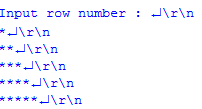
\includegraphics{fig/JT04fig}
				\end{figure}
			
			\item 解題思維:
			\subitem 
				這題需要使用雙重for迴圈。第一個迴圈計算現在要印第幾列,第二個迴圈計算要印幾個星。
			\item 程式碼:
			\begin{cppcode}
				#include <stdio.h>
				
				int main()
				{
					int n, i, j;
					printf("Input row number : \n");
					scanf("%d", &n);
					for (i=1; i<=n; i++) { // 迴圈1:第i列
						for(j=0; j<i; j++) { // 迴圈2:印i個星
							printf("*");
						}
						printf("\n");
					}
					return 0;
				}
					
			\end{cppcode}
		\end{enumerate}

	\item 練習︰JP-010-2:印倒三角形(無空白)
		\begin{enumerate}
			\item 題目說明:
			\subitem 輸入正整數n<=20,輸出一個n層的倒三角形。
			\subitem 範例輸入:5
			\subitem 範例輸出:
			\begin{figure}[H]
				\centering
				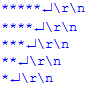
\includegraphics{fig/JP010fig}
			\end{figure}
			\item 解題思維:
			\subitem 印倒三角形時,第一列有n個星,下一列有n-1個星,以此列推,每換一列就少一個星,所以這題是要使用for迴圈來倒數。
\begin{comment}
			\item 程式碼:
			\begin{cppcode}
			#include <cstdio>
			
			int main()
			{
				int n, i, j;
				scanf("%d", &n);
				for (i=n; i>0; i--) { // 迴圈1:計算此列有i個星
					for(j=i; j>0; j--) { // 迴圈2:印出i個星
						printf("*");
					}
					printf("\n");
				}
				return 0;
			}
				
			\end{cppcode}
\end{comment}
		\end{enumerate}
	
	\item 挑戰︰JT-40印等腰三角形
		\begin{enumerate}
			\item 題目說明:
			\subitem 輸入N,印出一個N列的等腰三角形,其中第I列有2*I-1個\#,如程式範例結果所示。
			\subitem 範例輸入:5
			\subitem 範例輸出:
			\begin{figure}[H]
				\centering
				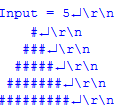
\includegraphics{fig/JT40fig}
			\end{figure}
			
			\item 解題思維:
			\begin{enumerate}
				\item 因為要印出N列,所以先寫一個執行N次的for迴圈,用變數row來計算現在是第幾列。
				\item 第row列要印出(n-row)個``空白",及(2*row-1)個``\#",所以分別用兩個for迴圈印``空白"及``\#"。
			\end{enumerate}
\begin{comment}			
			\item 程式碼:
			\begin{cppcode}
				#include <stdio.h>
				
				int main()
				{
					int i, row, n;
					scanf("%d", &n);
					printf("Input = %d\n", n);
					for (row=1; row<=n; row++) {
						for (i=0; i<n-row; i++) printf(" ");
						for (i=0; i<2*row-1; i++) printf("#");
						printf("\n");
					}
					return 0;
				}
				
			\end{cppcode}
\end{comment}
		\end{enumerate}

\end{enumerate}

%\subsubsection {do while {\color{blue}(若有多餘時間)}}


\section{函數}
\subsection{printf()格式輸出}
\begin{enumerate}
	\item 講解︰JB-02:九九乘法表
		\begin{enumerate}
			\item 題目說明:
			\subitem 印出如輸出之九九乘法表。
			\begin{figure}[h]
				\centering
				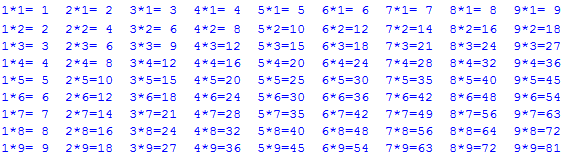
\includegraphics[width=12cm]{fig/JB02fig}
			\end{figure}
			\item 解題思維:
			\begin{enumerate}
				\item 先看第一列,會變動的數是``被乘數",而且變動是有規律的1,2,3...,9,所以我們寫一個會執行9次的for迴圈,讓變數j從1跑到9。變數j就是要輸出的``被乘數"。
				\begin{figure}[H]
					\centering
					
\includegraphics[width=12cm]{fig/JB02fig_2}
				\end{figure}
				\item 再來觀察``乘數",同一列的乘數是固定的,乘數隨著列改變,也就是說第i列的乘數是i。總共有9列,所以要寫一個會執行9次的for迴圈。變數i就是要輸出的``乘數"。
				\item ``乘積"只要將i, j 相乘就可以了。
				\item 這題使用printf()格式輸出比較容易。``\%2d"表示輸出時,會給這個整數兩給位數,當輸出的整數只有個位數的時候,十位數的位置會自動補上``空格"。
			\end{enumerate}
			
			\item 程式碼:
			\begin{cppcode}
			#include <cstdio>
			
			int main()
			{
				for (int i=1; i<=9; i++) {//第i列的乘數是i
					for(int j=1; j<=9; j++) {//每一列的被乘數j都從1~9
						printf("%d*%d=%2d  ", j, i, i*j);
					}
					printf("\n");
				}
				return 0;
			}
				
			\end{cppcode}
		\end{enumerate}
	
	\item 練習︰JA-007:九九乘法表 (兩排)
		\begin{enumerate}
			\item 題目說明:
			\subitem 印出九九乘法表,如輸出結果所示。
			\begin{figure}[h]
				\centering
				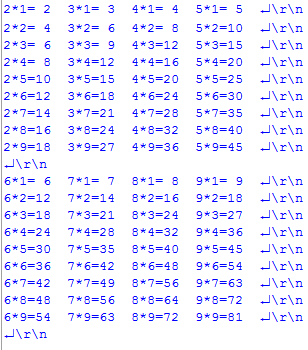
\includegraphics[height=6cm]{fig/JA007fig}
			\end{figure}
			\item 解題思維:
			\subitem 可以想成輸出兩個大群組的九九乘法表,當輸出第r (r=0, 1) 個群組時``被乘數"$=j+r\times4.$ (j=2, 3, 4, 5)。
\begin{comment}			
			\item 程式碼:
			\begin{cppcode}
				#include <cstdio>
				
				int main()
				{
					for (int r=0; r<2; r++) {//兩個群組
						for (int i=1; i<=9; i++) {//第i列的乘數是i
							for(int j=2; j<=5; j++) {//被乘數=j+r*4
								printf("%d*%d=%2d  ", j+r*4, i, i*(j+r*4));
							}
							printf("\n");
						}
						printf("\n");
					}
					return 0;
				}
				
			\end{cppcode}
\end{comment}
		\end{enumerate}
	
\end{enumerate}
\subsection{自訂函數}
\begin{enumerate}
	\item 講解︰JT-04印三角形函數
	\begin{enumerate}
		\item 題目說明:
		\subitem 輸入N,印出N列的星號(*),其中第I列有I個星,如執行範例所示。
		\subitem 範例輸入:5
		\subitem 範例輸出:
		\begin{figure}[H]
			\centering
			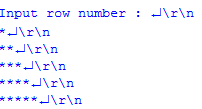
\includegraphics{fig/JT04fig}
		\end{figure}
		
		\item 解題思維:
		\begin{enumerate}
			\item 自己定義畫三角形的函數,使用這個函數時,需要輸入參數n,這樣函數才知道三角形有幾列。
			\item 將畫三角形的程式碼寫進函式裡,主程式main裡面只需要呼叫函數即可印出三角形。
		\end{enumerate}
		
		\item 程式碼:
		\begin{cppcode}
			#include <stdio.h>
			
			void triangle(int n);
			
			int main()
			{
				int n;
				printf("Input row number : \n");
				scanf("%d", &n);
				triangle(n);
				return 0;
			}
			
			void triangle(int n)
			{
				int i, j;
				for (i=1; i<=n; i++) {
					for (j=0; j<i; j++) { printf("*"); }
					printf("\n");
				}
			}
			
		\end{cppcode}
	\end{enumerate}
	
	\item 練習︰JP-010-2:印倒三角形(無空白)
	\begin{enumerate}
		\item 題目說明:
		\subitem 輸入正整數n<=20,輸出一個n層的倒三角形。
		\subitem 範例輸入:5
		\subitem 範例輸出:
		\begin{figure}[H]
			\centering
			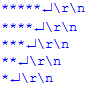
\includegraphics{fig/JP010fig}
		\end{figure}
		\item 解題思維:
		\begin{enumerate}
			\item 自己定義畫三角形的函數,使用這個函數時,需要輸入參數n,這樣函數才知道三角形有幾列。
			\item 將畫倒三角形的程式碼寫進函式裡,主程式main裡面只需要呼叫函數即可印出三角形。
		\end{enumerate}
\begin{comment}
		\item 程式碼:
		\begin{cppcode}
			#include <cstdio>
			
			void plot(int n);
			
			int main()
			{
				int n;
				scanf("%d", &n);
				plot(n);
				return 0;
			}
			
			void plot(int n)
			{
				int i, j;
				for (i=n; i>0; i--) {
					for(j=i; j>0; j--) {
						printf("*");
					}
					printf("\n");
				}
			}		
		\end{cppcode}
\end{comment}
	\end{enumerate}
	
	\item 練習︰JT-40:印等腰三角形
		\begin{enumerate}
			\item 題目說明:
			\subitem 輸入N,印出一個N列的等腰三角形,其中第I列有2*I-1個\#,如程式範例結果所示。
			\subitem 範例輸入:5
			\subitem 範例輸出:
			\begin{figure}[H]
				\centering
				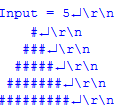
\includegraphics{fig/JT40fig}
			\end{figure}
			
			\item 解題思維:
			\begin{enumerate}
				\item 自己定義畫三角形的函數,使用這個函數時,需要輸入參數n,這樣函數才知道三角形有幾列。
				\item 將畫等腰三角形的程式碼寫進函式裡,主程式main裡面只需要呼叫函數即可印出三角形。
			\end{enumerate}
\begin{comment}			
			\item 程式碼:
			\begin{cppcode}
				#include <stdio.h>
				
				void plot(int n);
				
				int main()
				{
					int n;
					scanf("%d", &n);
					printf("Input = %d\n", n);
					plot(n);
					
					return 0;
				}
				
				void plot(int n)
				{
					int i, row;
					for (row=1; row<=n; row++) {
						for (i=0; i<n-row; i++) printf(" ");
						for (i=0; i<2*row-1; i++) printf("#");
						printf("\n");
					}
				}
				
				
			\end{cppcode}
\end{comment}
		\end{enumerate}
		
	
	
	\item 挑戰︰JT61:Game Over
		\begin{enumerate}
			\item 題目說明:
			\subitem 輸入整數 m 和 n,輸出以 \# 排成框,中間為 Game Over 之圖案,其中 m 為 G 之
			前和 r 之後與邊界的空格數,n 為文字與上下邊界的空格數。例如輸入 2 1,則輸出為
			\begin{figure}[h]
			\centering
			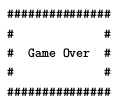
\includegraphics{fig/game_over_fig}
			\end{figure}
			\item 解題思維:
			\begin{enumerate}
				\item 第1列有11+2m個\#。
				\item 接下來n列頭尾是\#,中間有9+2m個空白。
				\item 再下一列是\#加m個空白,加Game Over,加m個空白和\#。
				\item 接下來n列頭尾是\#,中間有9+2m個空白。
				\item 最後一列有11+2m個\#。
			\end{enumerate}
\begin{comment}
			\item 程式碼:
		\begin{cppcode}
			#include <iostream>
			
			using namespace std;
			
			int main()
			{
				int m, n;
				cin >> m >> n;
				for (int i=0; i<11+2*m; i++) cout << "#"; // Row 1
				cout << endl;
				for (int r=0; r<n; r++) { // Next n rows
					cout << "#";
					for (int i=0; i<9+2*m; i++) cout << " ";
					cout << "#" << endl;
				}
				cout << "#"; // Middle row
				for (int i=0; i<m; i++) cout << " ";
				cout << "Game Over";
				for (int i=0; i<m; i++) cout << " ";
				cout << "#" << endl;
				for (int r=0; r<n; r++) { // Next n rows
					cout << "#";
					for (int i=0; i<9+2*m; i++) cout << " ";
					cout << "#" << endl;
				}
				for (int i=0; i<11+2*m; i++) cout << "#"; // Last row
				cout << endl;
				return 0;
			}
		
	\end{cppcode}
\end{comment}				
		\end{enumerate}
	
\end{enumerate}



\section{遞迴}

\subsection{遞迴}
\begin{enumerate}
	\item 講解:JA-008:遞迴解1+2+...+n
		\begin{enumerate}
			\item 題目說明:
			\subitem 使用遞迴方式算出 1+2+...+n
			
			\item 解題思維:
			\subitem 假設$f(n)=1+2+...+n$,則遞迴的計算方法為$f(n)=n+f(n-1)$。
			
			\item 程式碼:
			\begin{cppcode}
				#include <cstdio>
				
				int f(int n);
				
				int main()
				{
					int n;
					scanf("%d", &n);
					printf("%d", f(n));
					return 0;
				}
				
				int f(int n)
				{
					if (n==1) return 1;
					return n + f(n-1);
				}
								
			\end{cppcode}
		\end{enumerate}
	
	\item 練習:A059:遞迴計算n階乘
		\begin{enumerate}
			\item 題目說明:
			\subitem 輸入一正整數N,輸出N!。其中$N! = 1\times2\times3\times...\times N$
			
			\item 解題思維:
			\subitem 假設函數$fact(n)=n! $,其遞迴的計算方式為$fact(n)=n\times fact(n-1)$。
\begin{comment}			
			\item 程式碼:
			\begin{cppcode}
				#include<iostream>
				using namespace std;
				
				int fact(int n);

				int main()
				{
					int n;
					cin >> n;
					cout << fact(n);
					return 0;
				}

				int fact(int n)
				{
					if (n) return n * fact(n-1);
					else return 1;
				}

			\end{cppcode}
\end{comment}
		\end{enumerate}
	
	\item 講解:A029︰費式數列
		\begin{enumerate}
			\item 題目說明:
			\subitem 費氏數列定義如下 $f(0)=0, f(1)=1, f(n)=f(n-1)+f(n-2)$。
			題目是從螢幕輸入一個正整數 n,輸出 $f(n)$。
			
			\item 解題思維:
			\begin{enumerate}
				\item 本題可用遞迴或非遞迴方式計算。
				\item 因為程式簡明易了,可直接觀看程式碼尋求理解。
			\end{enumerate}
			
			\item 程式碼:
			\begin{cppcode}
				#include <stdio.h>

				int f(int n);

				int main()
				{
					int n;
					scanf("%d", &n);
					printf("%d", f(n));
					return 0;
				}

				int f(int n)
				{
					if (n<2) return n;
					return f(n-1)+f(n-2);
				}
			\end{cppcode}
		\end{enumerate}
	
	\item 挑戰:JA-009:爬樓梯有幾種爬法
		\begin{enumerate}
			\item 題目說明:
			\subitem 小明爬樓梯,已知要爬的梯數有N階,但小明一次可以爬1~3階,請問總共有幾種爬法?
			
			\item 解題思維:
			\subitem
			當n=1, 2, 3時,分別有1, 2, 4種爬法,當n>3時,爬樓梯的方法為$f(n)=f(n-1)+f(n-2)+f(n-3)$。
\begin{comment}			
			\item 程式碼:
			\begin{cppcode}
				#include <cstdio>
				
				int f(int n);
				
				int main()
				{
					int n;
					scanf("%d", &n);
					printf("%d", f(n));
					return 0;
				}
				
				int f(int n)
				{
					if (n==1) return 1;
					if (n==2) return 2;
					if (n==3) return 4;
					return f(n-1)+f(n-2)+f(n-3);
				}
			\end{cppcode}
\end{comment}
		\end{enumerate}
	
	\item 講解:JB-04︰河內塔
	\begin{enumerate}
		\item 題目說明:
		\subitem 依課堂上講解之河內塔規則,從柱1移到柱3,柱2為輔助。輸入環的個數n,輸出所有移動過程。
		
		\item 解題思維:
		\subitem 河內塔的解法如下:
		\begin{enumerate}
			\item 當只有1個環的時候,直接把環搬到目標柱子上。
			\item 當有n個環的時候
			\begin{enumerate}
				\item 先將(n-1)層的河內塔搬到輔助的柱子上。
				\item 接著將第n個環搬到目標柱子上。
				\item 最後,再將(n-1)層的河內塔從輔助的柱子搬到目標柱子上。 
			\end{enumerate}
			
		\end{enumerate}
		
		\item 程式碼:
		\begin{cppcode}
			#include <iostream>
			
			using namespace std;
			
			void hanoi(int n, int from, int to, int buf);
			
			int main()
			{
				int n;
				cin >> n;
				hanoi(n, 1, 3, 2);
				return 0;
			}
			
			void hanoi(int n, int from, int to, int buf)
			{
				if (n==1) {
					cout << from << " => " << to << endl;
				} else {
				hanoi(n-1, from, buf, to);
				cout << from << " => " << to << endl;
				hanoi(n-1, buf, to, from);
			}
		}
	\end{cppcode}
\end{enumerate}

	
	
	
	
\end{enumerate}

\section{8/17(四)下午:陣列}

\subsection{陣列}
\begin{enumerate}
	\item 講解:A030︰百數反印
		\begin{enumerate}
			\item 題目說明:
			\subitem 輸入 100 個正整數,反向印出此 100 個數。
			
			\item 解題思維:
			\subitem 本題使用陣列儲存 100 個數,再反向印出即可,是很基本的題目。
			
			\item 程式碼:
			\begin{cppcode}
				#include<iostream>
				using namespace std;
				int main()
				{
					int data[100];
					for (int i=0; i<100; i++) cin >> data[i];
					for (int i=99; i>=0; i--) cout << " " << data[i];
					return 0;
				}
			\end{cppcode}
		\end{enumerate}
	
	\item 講解︰JT-30︰排序
		\begin{enumerate}
			\item 題目說明:
			\subitem 輸入N及N個數 (N<100),將N個數從小到大印出來。
			
			\item 解題思維:
			\subitem 本題是練習排序的演算法。基本上排序的演算法很多,以下程式使用\href{https://zh.wikipedia.org/wiki/%E5%86%92%E6%B3%A1%E6%8E%92%E5%BA%8F}{氣泡排序法},
			這也是最基本的排序演算法之一。在程式中,i 的範圍可以從 0
			到 n-2,或則倒過來從 n-1 到 1 也可以,基本上就是要執行 n-1 輪的意思,但是 i 的
			範圍寫法不同,j 的上限寫法也跟著(有)一些變化,這是在閱讀參考連結時,應注意的地
			方。
			
			\item 程式碼:
			\begin{cppcode}
				#include <stdio.h>
			
				int main()
				{
					int i, j, t, n, a[100];
					scanf("%d", &n);
					for (i=0; i<n; i++) scanf("%d", a+i);
					for (i=n-1; i>0; i--) {
						for (j=0; j<i; j++) {
							if (a[j]>a[j+1]) {
								t=a[j];
								a[j]=a[j+1];
								a[j+1]=t;
							}
						}
					}
					printf("%d", a[0]);
					for (i=1; i<n; i++) printf(" %d", a[i]);
					return 0;
				}
			\end{cppcode}
		\end{enumerate}
	
\end{enumerate}




\end{document}
